% mnras_template.tex
%
% LaTeX template for creating an MNRAS paper
%
% v3.0 released 14 May 2015
% (version numbers match those of mnras.cls)
%
% Copyright (C) Royal Astronomical Society 2015
% Authors:
% Keith T. Smith (Royal Astronomical Society)

% Change log
%
% v3.0 May 2015
%    Renamed to match the new package name
%    Version number matches mnras.cls
%    A few minor tweaks to wording
% v1.0 September 2013
%    Beta testing only - never publicly released
%    First version: a simple (ish) template for creating an MNRAS paper

%%%%%%%%%%%%%%%%%%%%%%%%%%%%%%%%%%%%%%%%%%%%%%%%%%
% Basic setup. Most papers should leave these options alone.
\documentclass[a4paper,fleqn,usenatbib]{mnras}

% MNRAS is set in Times font. If you don't have this installed (most LaTeX
% installations will be fine) or prefer the old Computer Modern fonts, comment
% out the following line
\usepackage{newtxtext,newtxmath}
% Depending on your LaTeX fonts installation, you might get better results with one of these:
%\usepackage{mathptmx}
%\usepackage{txfonts}

% Use vector fonts, so it zooms properly in on-screen viewing software
% Don't change these lines unless you know what you are doing
\usepackage[T1]{fontenc}
\usepackage{ae,aecompl}

\usepackage{mhchem}



\usepackage{graphicx}
\usepackage{subcaption}
\usepackage{float}
\usepackage{gensymb}
\usepackage{color}
\usepackage{booktabs,chemformula}
\usepackage[export]{adjustbox}

\usepackage{verbatim}
\usepackage{tabularx}

\usepackage{caption}
\usepackage{subcaption}
\usepackage{amsmath}

\usepackage{tikz}
\usepackage{hyperref}
\usepackage{longtable}
\usepackage{color}
\newcommand{\todo}[1]{\textcolor{red}{#1}}


\newcommand{\LamostGiants}{454180}
\newcommand{\project}[1]{\emph{#1}}
\newcommand{\lamost}{\project{LAMOST}}
\newcommand{\apogee}{\project{APOGEE}}

\newcommand{\tc}{\project{The Cannon}}

\newcommand{\teff}{T_{\rm eff}}
\newcommand{\logg}{\log_{10}[g\,({\rm cm\,s}^{-2})]}

%%%%%%%%%%%%%%%%%%% TITLE PAGE %%%%%%%%%%%%%%%%%%%

% Title of the paper, and the short title which is used in the headers.
% Keep the title short and informative.
\title[Mg-K anti-correlation in LAMOST]{Discovery of Mg-depleted and K-enhanced Stars in \textit{LAMOST}}

% The list of authors, and the short list which is used in the headers.
% If you need two or more lines of authors, add an extra line using \newauthor
\author[Kemp et al.]{Alex J. Kemp,$^{1}$\thanks{E-mail: ajkem1@student.monash.edu}
Andrew R. Casey,$^{1,2}$
Matthew T. Miles,$^{1}$
Brodie J. Norfolk,$^{1}$\newauthor
John C. Lattanzio,$^{1}$
Amanda I. Karakas,$^{1}$
Kevin C. Schlaufman,$^{3}$
Anna Y.~Q. Ho,$^{4}$\newauthor
Christopher A. Tout$^{1,5}$
%Melissa K. Ness,$^{5}$
%David W. Hogg,$^{6}$
\\
% List of institutions
$^{1}$School of Physics \& Astronomy, Monash University, Clayton 3800, Victoria, Australia\\
$^{2}$Faculty of Information Technology, Monash University, Clayton 3800, Victoria, Australia\\
$^{3}$Department of Physics and Astronomy, Johns Hopkins University, Baltimore, MD 21218, USA\\
$^{4}$Cahill Center for Astrophysics, California Institute of Technology, MC 249-17, 1200 E California Blvd, Pasadena, Ca, 91125, USA\\
$^{5}$Institute of Astronomy, Madingley Road, Cambridge CH30HA, United Kingdom
%$^{5}$ Max-Planck-Institut f$\ddot{u}$r Astronomie, K$\ddot{o}$nigsthul 17, D-69117 Heidelberg, Germany\\
%$^{6}$ Center for Cosmology and Particle Physics, Department of Physics, New York University, 4 Washington Pl., room 424, New York, NY, 10003, USA\\
}

% These dates will be filled out by the publisher
\date{Accepted 2018 XX XX. Received 2018 YY YY; in original form 2018 ZZ ZZ}

% Enter the current year, for the copyright statements etc.
\pubyear{2018}


\begin{document}
\label{firstpage}
\pagerange{\pageref{firstpage}--\pageref{lastpage}}
\maketitle

% Abstract of the paper
%The detailed chemical composition of a star acts as a fossil record of the conditions when it formed. 

\begin{abstract}
Stars with unusual elemental abundances offer clues about rare astrophysical events or nucleosynthetic pathways. Stars with significantly depleted magnesium and enhanced potassium (e.g., $[{\rm K}/{\rm Fe}] > 1$; $[{\rm Mg}/{\rm Fe}] < -0.5$) have to date only been found in the massive globular cluster NGC~2419, and to a lesser extent, NGC~2808. The origin of this abundance signature remains unknown, as does the reason for its apparent exclusivity to these two globular clusters. Here we present 112 field stars, identified from \LamostGiants\ \lamost\ giant stars, that show significantly enhanced [K/Fe] and depleted [Mg/Fe] abundance ratios.
Our sample spans a full range of metallicities ($-1.5 < [{\rm Fe}/{\rm H}] < 0.3$), yet none show abundance ratios of [K/Fe] or [Mg/Fe] that are as extreme as those observed in NGC~2419. 
\todo{We conclude what about the origin. What does this imply.}
This sample will help guide modelling attempts to explain the origin for the Mg-K abundance signature, which we show exists throughout the Milky Way.
\end{abstract}

% Select between one and six entries from the list of approved keywords.
% Don't make up new ones.
\begin{keywords}
methods: data analysis -- catalogues -- stars: chemically peculiar -- Galaxy: abundances -- Galaxy: evolution -- galaxies: globular clusters: individual: evolution
\end{keywords}

%%%%%%%%%%%%%%%%%%%%%%%%%%%%%%%%%%%%%%%%%%%%%%%%%%

%%%%%%%%%%%%%%%%% BODY OF PAPER %%%%%%%%%%%%%%%%%%

\section{Introduction}
\label{sec:intro}
NGC 2419 is the Milky Way's third most massive globular cluster, and its chemical composition makes it perhaps the most unusual star cluster in the Galaxy. Recent spectroscopic studies of red giant branch (RGB) stars in NGC 2419 revealed a strong anti-correlation between Mg and K abundances in nearly half of the studied stars, and weaker abundance relations in Si, Sc, Ca, Ti and V with Mg \citep{mucciarelli2012,cohenkirby2012}.

A targeted search looking for [K/Fe] in RGB and main sequence turn-off stars in other clusters (NGC 6752, NGC 6121, NGC 1904, 47 Tuc, NGC 6397, NGC 7099, and $\omega$ Centauri) and field stars concluded that all K abundance ratios fell within the bounds of the Mg-normal population in NGC 2419 \citep{carretta2013}. 
NGC 2808 is the only cluster other than NGC 2419 where an anticorrelation between Mg and K has been observed. All 4 of NGC 2808's known Mg-depleted stars show an anti-correlation with K \citep{mucciarelli2015}, although the amplitude of these abundance ratios is far weaker than that in NGC 2419. The fact that the Mg-K anti-correlation is apparently confined to these two globular clusters would imply either a small population of unusual polluter stars, or a single extremely massive polluter star.

%Recently \cite{youngwooklee} used a Ca filter to identify two population in NGC 2419 corresponding to two generations of stars: G1, first generation metal poor stars, and G2, second generation stars displaying enhanced Ca and significantly increased He abundance ($\Delta Y = 0.19$). The Mg-depleted population identified previously was found to be contained with the G2 population.


An early modelling attempt at replicating the anomalous Mg/K abundance ratios assumed hot-bottom burning in AGB and super-AGB (SAGB) stars. \cite{ventura2012} succeeded in reproducing the Mg-K anti-correlation through the nuclear reaction pathway \ce{^{36}Ar(p,\gamma)^{37}K(\beta ^+ \nu)^{37}Ar(e^-,\nu)^{37}Cl(p,\gamma)^{38}Ar(p,\gamma)^39K} (corrected as per \cite{iliadis2016}) for the production of K. However, abundance patterns consistent with NGC 2419 were only possible if the Ar-K reaction cross section was increased to 100 times the laboratory value. or if the temperature at the base of the envelope could be made to exceed $\sim$150\,MK.

A more recent attempt to replicate the Mg/K abundance signature in NGC 2419 by \cite{iliadis2016} also targetted abundances of Si, Sc, Ca, Ti and V, elements reported as having weak correlations with Mg by \cite{cohenkirby2012}. The ultimate goal was to constrain the temperatures and densities required to produce the chemical signature, and thereby provide insight into potential polluters.\footnote{It is perhaps noteworthy that \cite{iliadis2016} identified a different main reaction pathway for K nucleosynthesis to that of \cite{ventura2012}, which is relegated to a minor secondary pathway. The main pathway \cite{iliadis2016} identify is \ce{^{36}Ar(p,\gamma)^{37}K(\beta ^+ \nu)^{37}Ar(p,\gamma)^{38}K(\beta ^+ \nu)^{38}Ar(p,\gamma)^39K}.}
Unless extremely high densities were invoked ($>10^8\,{\rm g\,cm}^{-3}$), it was found that temperatures between 100 and 200\,MK were necessary. This constraint rules out many pollution sites, including: core and shell burning of low-mass stars, high-mass and super-massive stars, as well as regular AGB stars. Super-AGB (SAGB) stars, however, were considered as potential candidates, with only a relatively small (roughly 10-20 MK) increase in temperature required to fall in the acceptable band of parameter space identified. The other potential candidate identified were novae, although the lack of detailed models of white dwarf accretion of metal-poor material adds considerable uncertainty. However, based on current nova frequency in globular clusters determined by \cite{kato2013novae}, \cite{iliadis2016} conclude that the amount of material that would be produced by novae is at most 1\% of the total required mass to pollute 30\% of NGC 2419.

Another proposed  polluter candidate is a pair-instability super nova \citep[PISN;][]{carretta2013}. Unique to extremely massive Population III stars, these events involve the total destruction of the star, with no black hole remnant left behind. The main argument for this idea is that the extreme rarity of these events, coupled with the huge masses of processed material released, could allow for the abundance signature in NGC 2419 to be the result of a single, extremely rare event, which would explain why it is not seen in any other globular clusters. However, the signature odd-even proton number abundance pattern associated with PISNs is absent from NGC 2419 \citep{cohenkirby2012}, making this particular scenario unlikely.

%It has been suggested that NGC 2419's position and size, being both very massive and very distant from the Milky Way compared to many other globular clusters, aids it in retaining enriched material from explosive events \citep{mucciarelli2012}. It is also perhaps noteworthy that NGC 2808 is also one of the more massive globular clusters of the Milky Way, although it is far closer to the Galactic Centre. But if this unknown pollution event is common among globular clusters and the cause of its apparent exclusivity to NGC 2808 and NGC 2419 is enhanced ejecta retention due to high mass, then other massive clusters such as $\omega$ Centauri would also be expected contain the signature, which to date has not been observed.

%While it is plausible that the increased mass and greater distance from the gaseous disk of the Milky Way would cause a clusters first generation polluter stars to have an increased effect on the second generation of stars, this effect would apply to all ejecta (assuming comparable energies). So while it might be expected that second generation stars in clusters similar to NGC 2419 made up of more material processed by the first generation than other lighter globular clusters, it doesn't explain why the ejecta from the first generation was apparently dominated by this as yet unknown polluter object resulting in the Mg-K anti-correlation. In the opinion of the author, it is the identity and physical characterisation of this unknown polluter that is of the greatest scientific interest, with such a result also hopefully answering the question of the signatures uniqueness.


One  mechanism for [Mg/Fe] depletion is the introduction of $\alpha$-poor and Fe-rich material released from Type Ia supernovae \citep{tsujimoto2012first} which locally pollutes the `normal' [Mg/Fe] ratios that arise from Type II supernovae. However, the two populations in NGC 2419 are indistinguishable in their [Fe/H] abundance \citep{cohenkirby2012}. Furthermore, Type Ia supernovae enrichment cannot account for the enhanced K abundance observed in NGC 2419. In fact, K is hard to make in sufficient quantities anywhere without invoking unrealistic temperature conditions or increasing reaction rates from measured values by several orders of magnitude \todo{[citations]}. Another mechanism for reducing [Mg/Fe] is through the Mg-Al nucleosynthetic chain in high temperature hydrogen burning. However, no Al correlation is observed with the Mg depletions in NGC 2419 \citep{cohenkirby2012,mucciarelli2012}.

Beyond the intrinsic scientific value of identifying the responsible mechanism for the puzzling Mg-K anti-correlation, a satisfactory explanation for the Mg-K signature could offer insight into the underestimation of K abundances in the Milky Way predicted by galactic chemical evolution models \citep{kobayashi2011}. Recent work by \cite{ritter2017} on K production in O-C shell mergers shows promise as an alternative source of K. Identifying the source of the Mg-K anti-correlation could also be beneficial to efforts to understand globular cluster formation and evolution.

Here we use \lamost\ data to conduct the largest ever search for stars enhanced in potassium and depleted in magnesium. The discovery (or non-discovery) of such stars will guide models that attempt to explain the Mg-K anti-correlation and related abundance phenomena. In particular, the search should provide strong evidence for the uniqueness of the mysterious site of nucleosynthesis responsible for the pattern to globular clusters, or lack thereof. In Section \ref{sec:method} we outline our methods to identify candidates enhanced in K and depleted in Mg, and the follow-up observations and abundance analysis of those candidates. In Section \ref{sec:discussion} we discuss our results and their implications for possible pollution mechanisms. Section \ref{sec:conclusion} summarises the main results.


%This study, which queries \LamostGiants\ \lamost\ giants for depleted Mg and enhanced K, seeks to provide additional information which can be used to guide and test models attempting to explain the Mg-K anti-correlation and related phenomena. The large sample size provides greater insight into the supposed exclusivity of the signature, and the stars identified present an important opportunity for follow up observations.


\section{Method \& Observations}
\label{sec:method}
\subsection{Candidate selection from \lamost\ spectra}
We used a set of \LamostGiants\ giant stars from the second \lamost\ data release. The spectra were placed at rest-frame on a common wavelength sampling from 3905\,\AA\ to 9000\,\AA\ and pseudo-continuum-normalised by \citet{ho2017}. \tc\ \citep{ness2016,ho2017} was used to estimate effective temperature ($\teff$), surface gravity ($\logg$), metallicity ([Fe/H]), and mean $\alpha$-element abundance relative to iron ([$\alpha$/Fe]) using 9,952 stars in common between \lamost\ and the \apogee\ \citep{alam2015} survey, through the use of a data-driven spectral model. Unless otherwise stated, these transferred labels are those referred to throughout this study. For details regarding the preparatory work, model generation, and label transfer between the \apogee\ and \lamost\ surveys, we direct the reader to \citet{ho2017}. 

We identified potential Mg-depleted and K-enhanced stars by searching for significant deviations in residual flux. The flux residuals were taken as the normalised \lamost\ flux and the best-fitting data-driven model from \tc\ (where $f_{\textrm{residual}} = f_{\textrm{data}} - f_{\textrm{model}}$). A positive residual implies a higher observed normalised flux than expected by the model (less stellar absorption than predicted by the model), while a negative residual implies a lower observed normalised flux than expected (more stellar absorption than predicted by the model). Figure \ref{fig:posterchild} shows the \lamost\ spectra, and best-fitting model from \tc, for candidate J034458.82+592955.1.

We fit a gaussian profile to the flux residuals for all three absorption lines in the Mg triplet (5167\,\AA, 5172\,\AA, 5184\,\AA) as well as the K doublet (7665\,\AA, 7699\,\AA) for all \LamostGiants\ giants. For each star we recorded the profile amplitudes, wavelengths, widths, as well as associated measurement uncertainties of these quantities. We identified candidates by requiring they match at least one of the following three quality filters:
\begin{enumerate}
\item We required the amplitude $A$ of the profile at the Mg 5184 \AA \ line to satisfy $A_{{\rm Mg} @ 5184} > 0.05$ and the amplitude of the profile at the K 7665 line to satisfy $A_{{\rm K}\,@\,7665} < -0.05$. Both amplitudes must also be measured at more than $3\sigma$ ($|A|/\sigma_{A} \geq 3$).
\item We required any two of the three Mg triplet lines to satisfy $A > 0.05$ and at least one K line to have $A < -0.05$, and for those amplitudes to have $|A|/\sigma_{A} \geq 3$.
\item We required any two of the three Mg triplet lines to have $A > 0$ and both K lines to have $A < 0$, and for the spectra to have a signal-to-noise ($S/N$) ratio of $S/N > 30$ in \lamost, and a reported $\chi_{r}^2 < 3$ from \tc.
\end{enumerate} 
 
These filters identified 384 unique stars. We visually inspected every candidate (multiple times) and excluded stars that showed any evidence of being a false positive, including candidates that exhibited data reduction issues, apparent absorption that was narrower than the expected spectral resolution, as well as 75 stars that exhibited chromospheric emission at H$\alpha$. The distilled catalogue contains 112 candidate stars enhanced in K and depleted in Mg.

We estimated [K/Fe] abundance ratios for all candidates by synthesising spectra to account for the flux residuals \citep{marcs,sme,vald,ispec}. We assume that absorption due to metals is accounted for by \tc, and deviations in flux around the potassium doublet is due to an increased [K/Fe] with respect to the model. We list estimated [K/Fe] abundance ratios in Table 1, where the error includes a 0.2\,dex systematic error floor that we have applied in quadrature with the fitting errors. We applied the same method to estimate [Na/Fe] from \lamost\ spectra. We note that while enhancements in [K/Fe] or [Na/Fe] can be estimated by synthesising the flux residuals, we cannot easily estimate [Mg/Fe] depletions in the same manner because it is difficult to separate the flux contribution of [Mg/Fe] (from [$\alpha$/Fe]) from the data-driven model. For this reason, we will adopt [$\alpha$/Fe] as a conservative upper limit for [Mg/Fe].



%\todo{The presence of Na enhancements were visually estimated from the sample of 112 candidate stars' flux spectra. Flux-based estimates placed at most 40 of the 112 stars (35\%) as being likely Na enhanced targets.} Na abundances calculated from the \lamost\ spectra later revealed 30\% of the target stars with [Na/Fe] above 0.5 dex. \todo{@andy add anything specific to Na abundance methods from LAMOST}.


\subsection{Follow-up observations with Magellan/MIKE}
High resolution spectra of three of the candidate stars selected based on observability (J075043.12+204658.0, J120032.60+024438.2 and J091825.49+172114.5) were obtained using Magellan/MIKE. \todo{@andy add relevant info on abundance calculations.}


\begin{figure*}
	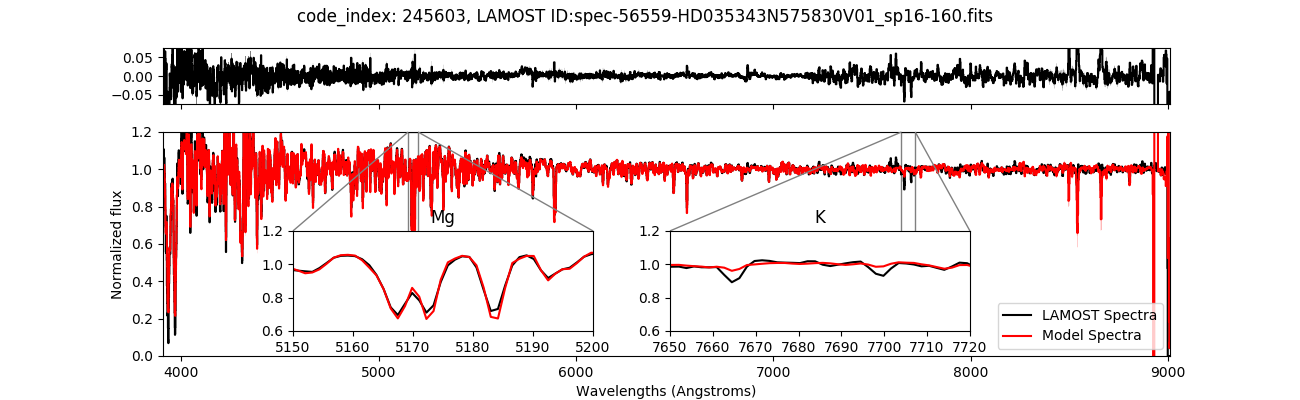
\includegraphics[width=\textwidth]{posterchildof13.png}
    \caption{Pseudo-continuum-normalised \lamost\ spectra for the Mg-depleted and K-enhanced candidate J034458.82+592955.1. The data  are shown in black and the best-fitting data-driven model from \tc\ is shown in red. We show zoom-in axes around the magnesium triplet and potassium doublet, which we used to identify Mg-K candidates. Note that $[\alpha/{\rm Fe}$ is a label in \tc\ model used, and J034458.82+592955.1 shows Mg depletions relative to the estimated [$\alpha$/Fe] value.}
    \label{posterchild}
\end{figure*}

\begin{figure}
	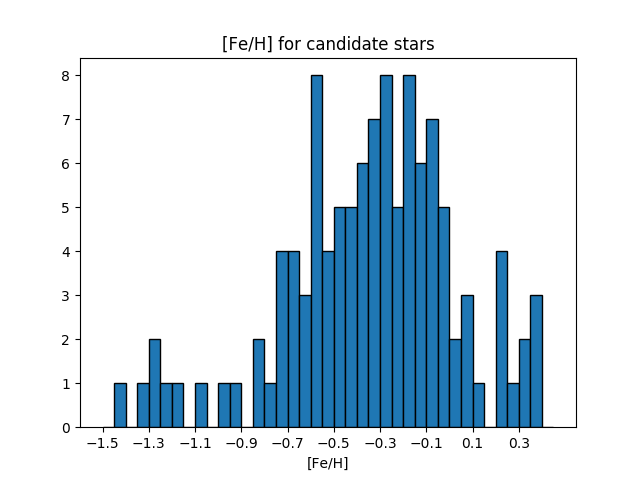
\includegraphics[width=\columnwidth]{histof113.png}
    \caption{Metallicity distribution for all 112 candidate stars identified with K-enhancement and Mg-depletion.}
    \label{mhist}
\end{figure}

\begin{figure}
	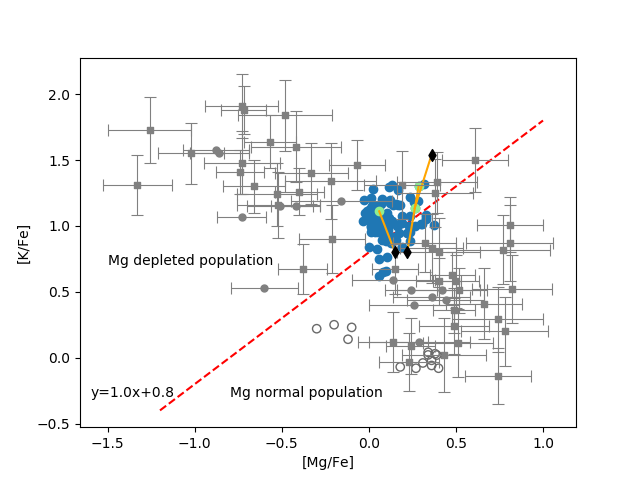
\includegraphics[width=\columnwidth]{Kvsmgmod.png}
    \caption{Comparison of [K/Fe] vs [$\alpha$/Fe] for the candidate stars with [K/Fe] vs [Mg/Fe] abundances for NGC 2419 and NGC 2808 \citep{cohenkirby2012, mucciarelli2012, mucciarelli2015}. See text for discussion on the use of [$\alpha$/Fe] as a proxy for [Mg/Fe]. The dotted line is arbitrary, and is present simply as a visual aide.}
    \label{KvsMg}
\end{figure}

\begin{figure}
	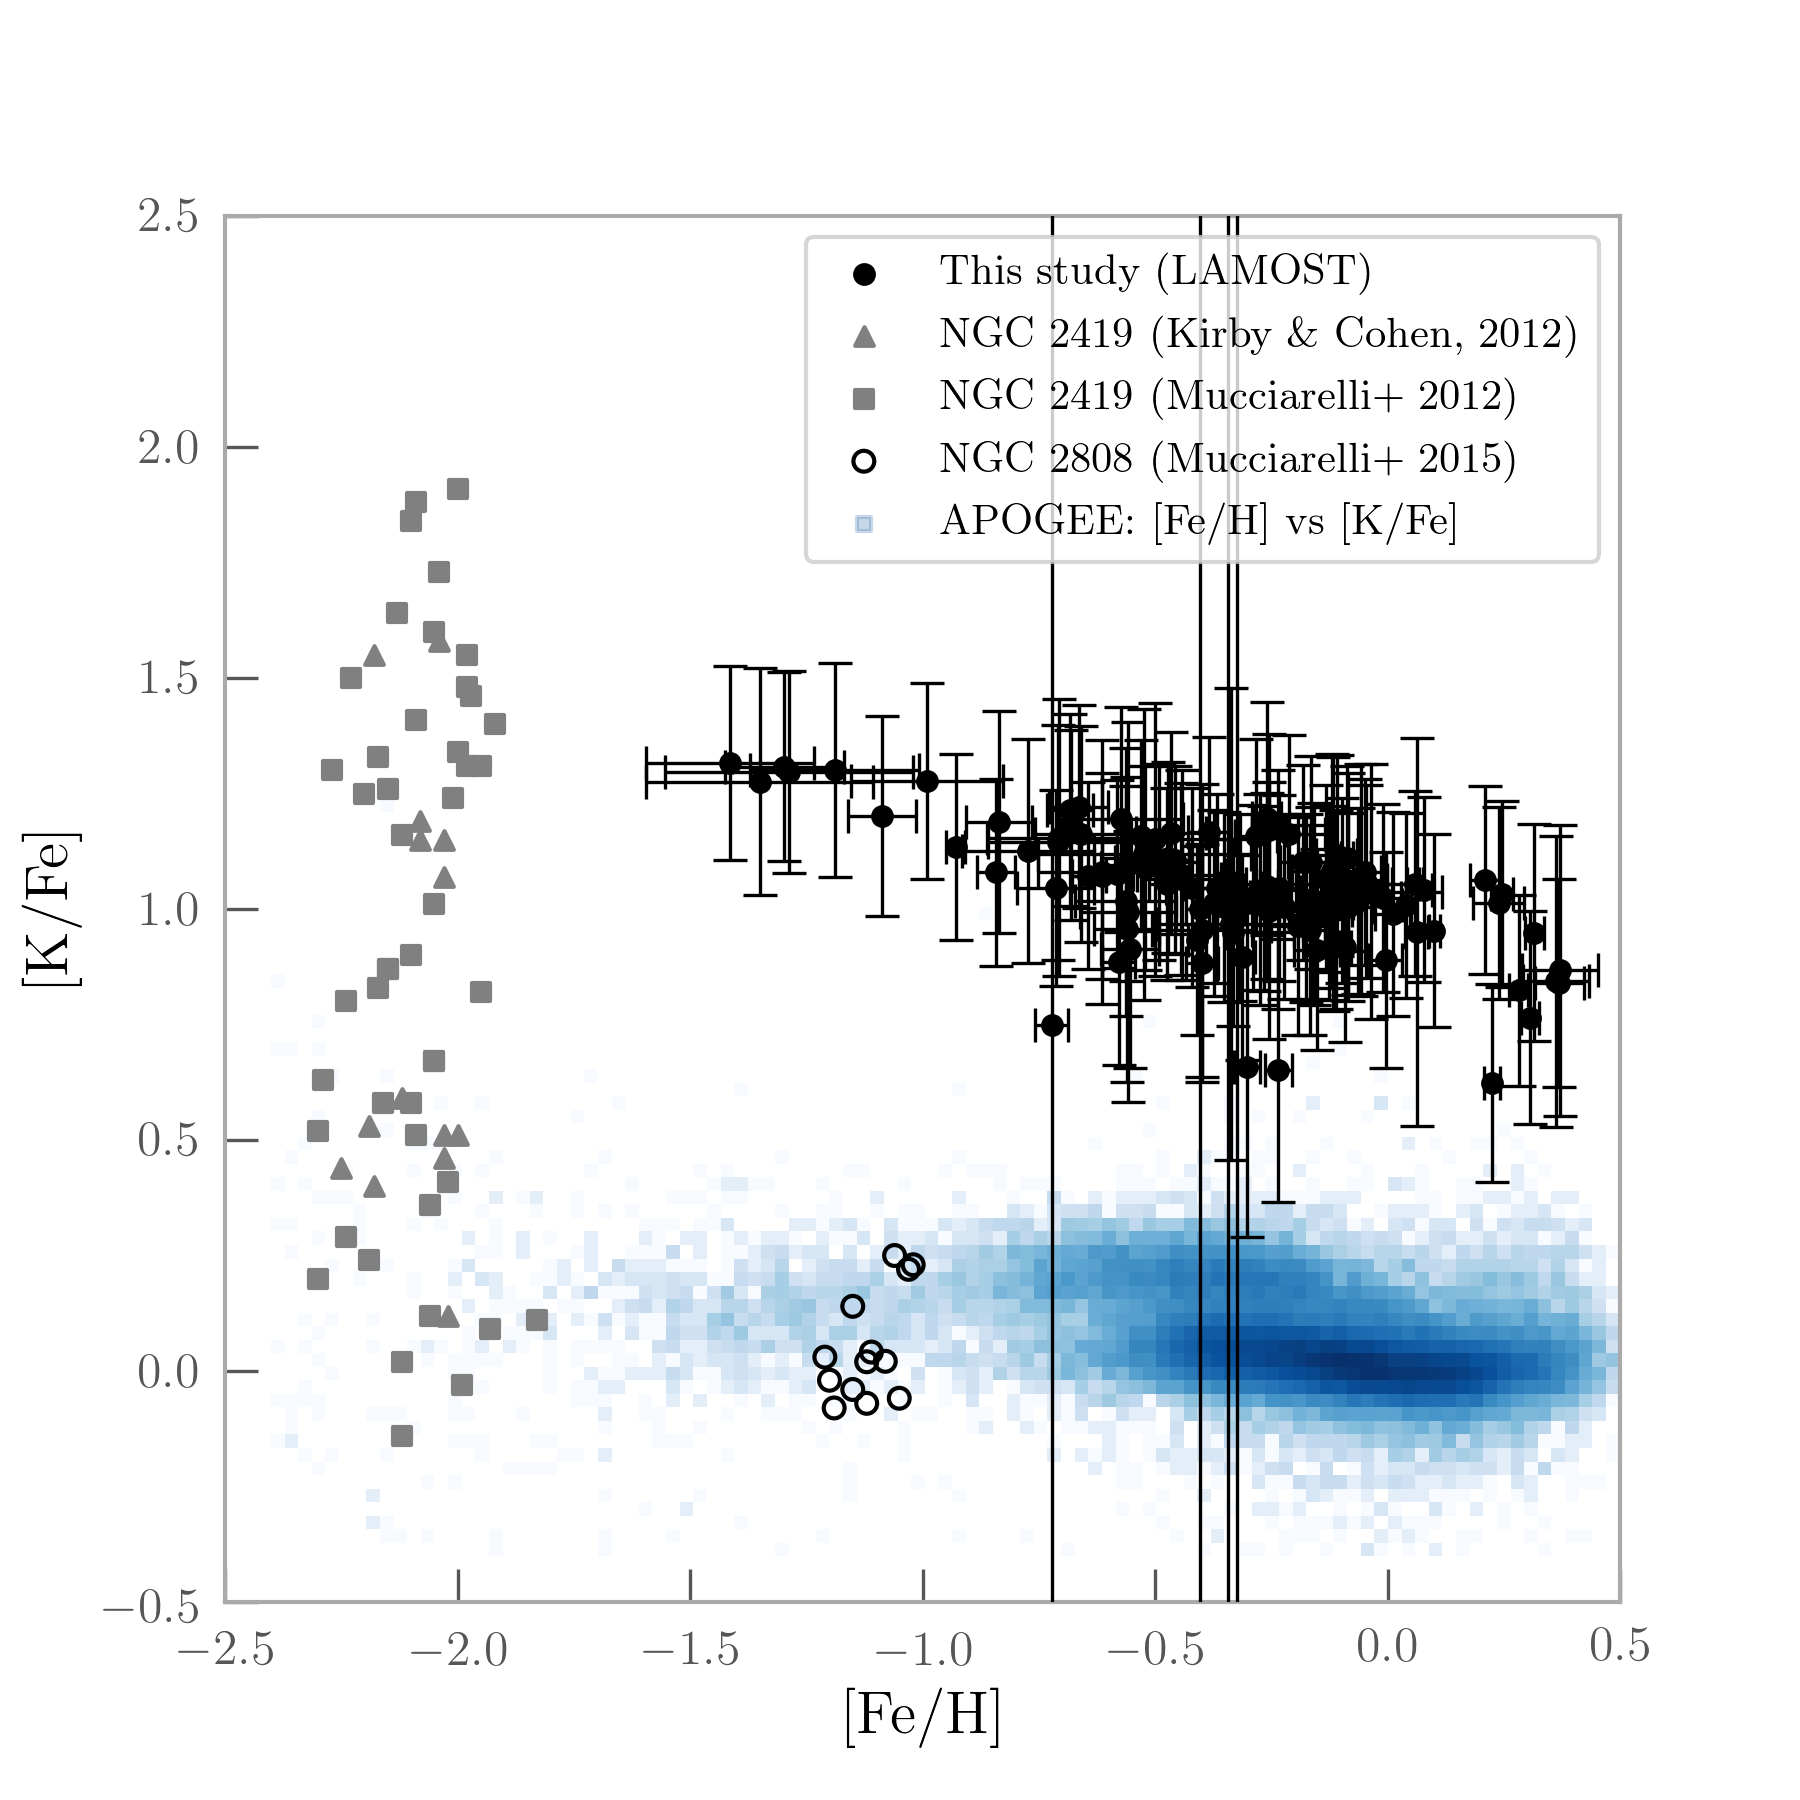
\includegraphics[width=\columnwidth]{KvsFe.png}
    \caption{[K/Fe] vs [Fe/H] for the candidate stars, overlaid with [K/Fe] vs [Fe/H] for NGC 2419 and NGC 2808 \citep{cohenkirby2012, mucciarelli2012, mucciarelli2015}. Metalicities for NGC 2808 are taken as the average metalicity for the cluster from \citet{harris1996}, as individual metallicities for these stars were not available.}
    \label{KvsFe}
\end{figure}

\section{Discussion}
\label{sec:discussion}

\subsection{Selection effects}
\label{sec:selectioneffects}
\cite{ho2017}'s sample of \lamost\ giants carries with it certain selection effects as a result of both the \textit{APOGEE} DR12 and \lamost\ samples. Metal poor stars with [Fe/H] $\lesssim-2$ are mostly absent from the sample as they were likely too dissimilar to the training stars for label transfer from \textit{APOGEE}. Unfortunately, the target selection process for \lamost\ is non-invertible, and so selection effects present in \lamost\ are not considered here beyond comparing the candidate stars' metallicity distribution with that of \cite{ho2017}.  The candidate stars are distributed across the entire giant branch, implying the abundance signature is not associated with any single particular stage in evolution, and that the chemical pattern is not due to a violation of the assumption of local thermodynamic equilibrium.

\subsection{Association with known globular clusters}
\label{sec:globclustasoc}
We cross-matched our candidates against a catalog of all known globular clusters \citep{harris1996}. No candidates can be associated with NGC~2419 or NGC~2808. The closest candidate to any globular cluster is J074807.22+261514.2, which lies 2.54\degree\ from Ko~2 \citep{koposov2007}. The large association and relatively  high metallicity of J074807.22+261514.2 ($[{\rm Fe}/{\rm H}] = -0.24$) make it highly unlikely to be a member. 

The spread in metallicity (Figure \ref{mhist}) is consistent with all candidates being field stars. The distribution reflects the original \LamostGiants\ sample of giants from which the candidates were selected.
No candidates have [Fe/H] $\sim -2$ -- the approximate metallicity of NGC 2419 -- nor are there many stars with [Fe/H] $\sim -1$ -- the metallicity of NGC 2808. Thus, we conclude that the candidates are not particular to any specific metallicity, including metallicities associated with NGC 2419 and NGC 2808.


\subsection{Detailed chemical abundances}
\label{sec:abundances}
Figure \ref{KvsMg} shows [K/Fe]  for the 112 star sample plotted against $[\alpha$/Fe] and overlaid with [K/Fe] from NGC 2419 and NGC 2808 plotted against [Mg/Fe] \citep{cohenkirby2012, mucciarelli2012, mucciarelli2015}. As described in Section \ref{sec:method}, we adopt [$\alpha$/Fe] as an upper limit for [Mg/Fe]. [K/Fe] vs [Mg/Fe] for the three stars from the sample observed using Magellan/MIKE is also shown. \todo{For these stars..}



%The use of $[\alpha$/Fe] to position the sample in \ref{KvsMg} is supported by the [Mg/Fe] measurements from the high-resolution spectra, which vary less than 0.1 dex from the level of $[\alpha$/Fe] for each of the relevant stars in the \lamost\ data. However, for the bulk of the sample decoupling [Mg/Fe] from $[\alpha$/Fe] is impossible, and so in general  we are unable to draw firm conclusions as to whether the sample exhibits anomalously low [Mg/Fe].

[K/Fe] for the candidate stars is generally lower than that of the Mg-depleted population in NGC 2419, but higher than that of the Mg-normal population. \todo{It is noteworthy that both of these populations identified in NGC 2808 have significantly lower levels of [K/Fe] than the candidate stars. --> What?}
Levels of [$\alpha$/Fe] fall within the lower limits of the Mg-normal population of both clusters, although as we are unable to decouple [Mg/Fe] from $[\alpha$/Fe] the exact level of Mg depletion for the candidates is unclear. The [Mg/Fe] abundances derived from Magellan/MIKE's high resolution spectra are consistent with the Mg-normal population in NGC 2419, although the small sample of these stars for which we have high resolution spectra means we are unable to confidently generalise this to the entire sample.

A similar relationship emerges when these abundances with typical galactic abundances for [K/Fe] and [Mg/Fe], taken from \cite{kobayashi2011}.
The sample's [K/Fe] appears definitively anomalous, with galactic values for [K/Fe] around $0.3 \pm 0.2$ dex, while the identified candidate stars have a spread in [K/Fe] from around 0.8-1.3. Note that the Magellan/MIKE abundance for candidate star J091825.49+172114.5 has [K/Fe] $=1.54$, confirming that at least some of the sample has extremely high levels of [K/Fe].

The candidate stars' [K/Fe] also exhibits an interesting anti-correlation with total metallicity, shown in Figure \ref{KvsFe}, \todo{which is absent from measurements in the Milky Way}. This may be consistent with a (somewhat) constant level of [K/H] between each star, which would then cause [K/Fe] to fall as [Fe/H] increases. It is interesting that the levels of [K/Fe] in the Mg-poor population of NGC 2419 appear consistent with this relation. \todo{make figure in python, add trend line}

%However, for reasons related to the use of both a data-driven model and a physical model for calculating abundances \todo{@andy add any elaboration on what the problem was, if necessary}, it is possible that this effect is an artefact of abundance processing rather than a physical relation. Without further observations of the sample stars, we are unable to say with certainty whether this phenomena is real or not.

The candidate stars' levels of [$\alpha$/Fe] were generally consistent with galactic levels of [Mg/Fe], as were the levels of [Mg/Fe] from the high resolution Magellan/MIKE spectra. Once again the inability to decouple [Mg/Fe] from $[\alpha$/Fe] means we are unable do draw firm conclusions about whether [Mg/Fe] is depleted relative to typical field stars, although the data we do have suggests not. No variation with metallicity is observed for [$\alpha$/Fe], including GCE effects relating of Type Ia supernovae enrichments.

%In contrast with the marked departure from galactic values for [K/Fe], [$\alpha$/Fe] varies from around 0-0.3 dex in the \lamost \ sample, similar to galactic levels of [Mg/Fe], which vary with metallicity from approximately 0.4$\pm$0.2 for [Fe/H] $\sim$ -1.5 to 0.1 $\pm$0.2 for [Fe/H] $\sim$ -0.3 \citep{kobayashi2011}. No variation with metallicity is observed within the \lamost sample's [$\alpha$/Fe].

[Na/Fe] was also measured for the \lamost\ data. Two distinct populations were observed, with a substantial minority of approximately 30\% of the sample having [Na/Fe] > 0.5, significantly higher than typical galactic abundances of [Na/Fe] $\lesssim$ 0.3 \citep{kobayashi2011}. However, this behaviour is very likely due to the effect of interstellar dust. This conclusion is based on values of E(B-V), taken from IRSA's all-sky dust map \citep{schlafly2011}, which were notably higher for the stars supposedly enriched in Na than for those consistent with galactic levels. \todo{It is worth mentioning briefly that the modelling work of \cite{prantzos2017} predicted an anti-correlation between Na and K in a 180 MK hydrogen burning environment appropriate to NGC 2808, while observational data for NGC 2808 implies a correlation between Na and K. For these newly identified candidate stars, no relation between Na and K abundance is observed.}

The implications of the calculated abundances are intriguing. The fact that from such a large sample of field stars none were found that replicated the extreme abundance pattern of NGC 2419 is strong evidence for the cluster's uniqueness regarding the extreme bi-modal nature of its abundance pattern. It is worth repeating however that the sample of \lamost\ giants searched had already been filtered of most of the stars that would have matched NGC 2419's metallicity.

The 112 star candidate pool of K enhanced stars represent a unique collection of stars; while not as K enhanced as the extreme population in NGC 2419, they exhibit K abundances well above typical galactic levels at a range of metallicities. It seems likely that whatever process is responsible for these anomalous field stars is similar to whatever caused the unusual stellar populations in NGC 2419 and NGC 2808.

\subsection{Impact scenarios regarding the Mg-K anti-correlation}

\label{sec:scenarios}
\begin{table*}
\centering
\caption{Tabulated data for 10 of the 112 candidate stars. Data for the full sample is available online.}
\label{data}
\begin{tabular}{cccccccccccccc}
\hline
\textbf{2MASSID} & \textbf{RA} & \textbf{DEC} & \textbf{S/N} & \textbf{V$_\textrm{r}$} & \textbf{T$_\textrm{eff}$} & $\boldsymbol \log{ \, \textbf{g}}$ & \textbf{{[}Fe/H{]}} & \textbf{{[}$\alpha$/Fe{]}} & \textbf{$\boldsymbol \chi_r ^\textbf{2}$} & \textbf{{[}K/Fe{]}} & \textbf{Error} & \textbf{{[}Na/Fe{]}} & \textbf{Error} \\ 
- & {[}deg{]} & {[}deg{]} & [pixel$^{-1}]$ & {[${\rm km\,s}^{-1}$]} & {[}K{]} & $[{\rm cm\,s}^{-2}]$ & {[}dex{]} & {[}dex{]} & - & {[}dex{]} & {[}dex{]} & {[}dex{]} & {[}dex{]} \\ \hline
J000908.89+124821.9 & 2.29 & 12.81 & 10 & -78.55 & 4892 & 2.82 & -0.12 & 0.33 & 0.19 & 1.08 & 0.16 & 0.86 & 0.12 \\
J002619.36+565612.1 & 6.58 & 56.94 & 31 & -39.57 & 4205 & 1.49 & 0.22 & 0.06 & 0.76 & 0.62 & 0.08 & 0.39 & 0.10 \\
J002907.61+354701.0 & 7.28 & 35.78 & 15 & -82.74 & 5116 & 3.56 & 0.24 & 0.17 & 0.18 & 1.01 & 0.06 & -0.20 & 0.00 \\
J003451.10+424543.0 & 8.71 & 42.76 & 15 & -79.15 & 4460 & 2.10 & -0.56 & 0.24 & 0.31 & 0.96 & 0.26 & -0.16 & 0.00 \\
J005649.98+391722.9 & 14.21 & 39.29 & 41 & -46.77 & 4578 & 2.67 & 0.31 & 0.10 & 0.44 & 0.76 & 0.11 & -0.02 & 0.00 \\
J010305.95+043445.9 & 15.77 & 4.58 & 90 & 20.69 & 4646 & 2.72 & 0.10 & 0.05 & 1.17 & 0.95 & 0.06 & -0.07 & 0.00 \\
J011949.36+063411.4 & 19.96 & 6.57 & 479 & -28.18 & 4820 & 2.61 & -0.29 & 0.09 & 2.38 & 1.03 & 0.00 & -0.04 & 0.00 \\
J013039.08+404843.8 & 22.66 & 40.81 & 71 & -80.34 & 4355 & 2.01 & -0.09 & 0.14 & 0.93 & 0.92 & 0.05 & 0.46 & 0.05 \\
J030101.42+560042.3 & 45.26 & 56.01 & 88 & -39.27 & 4878 & 2.53 & -0.32 & 0.09 & 0.67 & 1.00 & 8.70 & -0.02 & 0.00 \\
J032423.46+425429.6 & 51.10 & 42.91 & 23 & -56.74 & 4649 & 2.63 & -0.11 & -0.01 & 0.34 & 1.12 & 0.09 & 0.80 & 0.04 \\ \hline
\end{tabular}
\end{table*}


%Significantly enhanced [K/Fe] is rare; significantly enhanced [K/Fe] without an accompanying depletion of [Mg/Fe] is unknown. The candidate stars are also spread across a wide range of metallicities.

The spread in metallicities among our candidates is important to note. This implies that the process responsible for the Mg-K abundance signature is not necessarily tied to a certain epoch in the Milky Way's evolution. Rather, stars with enhanced K and depleted magnesium tend to form at all ages, across all metallicities. A hyper-massive Population III star may have been a plausible explanation for NGC~2419\todo{[CITATIONS NEEDED: WHO PROPOSED THIS]}, particularly given it's isolation from the Milky Way ($d_{GC} \approx 90\,{\rm kpc}$) and low metallicity. However, our discovery of Mg-K stars at all metallicities suggests against a hyper-massive Population III star as the polluter responsible.



As emphasized by \cite{prantzos2017}, a significant challenge presented by the signatures of NGC 2419 and NGC 2808 is obtaining both a depletion in Mg and an enhancement in K. Reducing Mg is possible through conversion of \ce{^{24}Mg} to \ce{^{27} Al} through Mg-Al chains at temperatures around 75 MK --  attainable in hot-bottom burning environments in AGB stars -- while it takes temperatures upwards of 150 MK to produce K -- temperatures potentially developed at the bottom of the convective envelope in SAGB stars \citep{iliadis2016}. This implies that the Mg depletion and K enrichment likely occur at separate sites, assuming a relatively simple hydrogen burning system.

Allowing different sites for Mg depletion and K enrichment, one scenario that could possibly produce a large K enhanced signature -- along with (inconsistently) depleted Mg and enhanced Na -- throughout the lifetime of the Milky Way would be a binary in which one of the stars is a SAGB star and the other is a less massive star. The scenario might proceed as follows:

The SAGB star produces K (destroying Na in the process \citep{prantzos2017}) which is then mixed throughout its envelope. It then deposits its K rich outer layers onto its smaller companion through wind-based accretion. This smaller companion would continue to evolve long after the SAGB star has formed a white-dwarf remnant and will, depending on its mass after accretion, either undergo hot-bottom burning or, more likely, will not. If the companion star had sufficient mass to undergo hot bottom burning, then Na could be produced \citep{prantzos2017}, with this material mixed throughout the envelope. In this scenario, it is observations of this smaller binary companion star that make up our sample of 112 giants.

Although this scenario allows for consistency with the total spread in metallicity, it doe not account for the uniqueness of the signal to NGC 2419 and NGC 2808 among globular clusters, nor does it satisfactorily explain why such a large proportion of stars in NGC 2419 exhibit the Mg-K anti-correlation. \todo{The idea that 30\% of the stars in NGC 2419 were once in a binary with SAGB stars is highly unlikely, to say the least.}

A direct test of this scenario would be whether at least most of the candidates are binaries with O-Ne white dwarf remnants, which would indicate that they could have formed SAGB binaries once.

The anti-correlation between [K/Fe] and [Fe/H] could be interpreted as a relatively constant level of [K/H] present in at least one region of star forming gas, resulting in a steady decrease in [K/Fe] as [Fe/H] increases. This interpretation is somewhat supported by the consistency of the relation with levels of [K/Fe] in NGC 2419. If this relation is real, we can perhaps -- without saying anything about the polluter star -- use it to motivate an evolutionary sequence that can account for observations of [K/Fe] and [Mg/Fe] both in NGC 2419 and our new 112 field star sample.

Suppose some unknown event(s) unique to very metal poor (possibly zero-metallicity) environments occurs. This event results in a gas cloud depleted in Mg and enhanced in K. The generation of stars that form directly from this gas carries this signature, and displays a significant reduction in Mg abundance and enhancement in K abundance similar to NGC 2419's extreme population. We will refer to this generation of stars Generation 1.

When the most massive stars of Generation 1 die, they release metals into the gas cloud, including significant amounts of Mg, which is formed in copious amounts in core-collapse supernovae, but \textit{not} K, which is very difficult to form in significant quantities. The [Mg/Fe] depletion originally carried in the cloud is much harder to detect in the next generation of stars forming from this material, Generation 2, due to the influx of Mg released by Generation 1. The K enhancement however remains (in principle) relatively easy to detect, having only been reduced relative to [Fe/H] by the total amount of iron released. As this cycle continues, [K/Fe] would continue to lower proportionately with the rate of iron release, while depletions in [Mg/Fe] would quickly become impossible to detect.

This cycle allows for the Mg depletions to be preserved in globular clusters, where even the most massive clusters only form at most 2 generations of stars. But it also allows the Mg signal to effectively be lost within the disc of the galaxy, where many generations of stars may form. Thus it provides a way of linking the current observations of our 112 candidate stars with the observations of NGC 2419. Certainly the idea that both groups of anomalous stars arise from the same polluter source must be entertained.

\todo{However, beyond the question of whether the [K/Fe]-[Fe/H] anti-correlation is real or not, the extreme difficulty of forming a cloud of Mg-depleted, K enriched material in the first place must be emphasized. Indeed, if we assume the primordial abundances (pre-mystery event) are similar to those of NGC 2419's Mg-normal population, then it is impossible. If the primordial cloud already has [Mg/Fe]$\approx 0.5$, to reduce this necessitates the addition of large amounts of iron rich material that is also very depleted in [Mg/Fe]. But as soon significant amounts of iron are added, [Fe/H] for the subsequent Mg-depleted population should increase, while no significant [Fe/H] variation between the two populations is observed \citep{cohenkirby2012, mucciarelli2012}. This implies that the mystery polluter star may have released its material into an environment enriched only by Big-Bang Nucleosynthesis (BBNS).}

Another issue facing the above scenario is that it requires a single gas cloud to form many generations of stars to be formed almost continously to be consistent with Figure \ref{KvsFe}. This is only known to occur in inside galaxies, which are massive enough and have sufficient gas to form multiple star forming regions. For smaller gas clouds, typically only one generation is formed before the remaining gas is lost through stellar winds. Although it is tempting to attempt to satisfy such concerns by allowing the stars to have formed some dwarf galaxy which then merged with the Milky Way, if the initial gas cloud increases so significantly in mass, then the difficulty of polluting such a cloud in the first place with such high levels of K increases proportionately.

More generally, the [K/Fe]-[Fe/H] anti-correlation observed is supportive of the origin of the Mg-K anti-correlation being temporally confined to an early epoch in the evolution of galaxies and globular clusters. However, this is not necessarily the only interpretation. For example, it could be that the K forming process is happening throughout the life of the galaxy, but the amount of K produced decreases with the metallicity of the polluter star, though there is no obvious reason why this would be the case.



\section{Conclusions}
\label{sec:conclusion}
Of the 454180 giant sample from \lamost, 112 candidate stars were identified as likely to have enhanced K and depleted Mg based on their absorption spectra. These stars show every appearance of being field stars, and they do not have the hallmarks of being the product of NLTE effects. The candidate sample reflected the metallicity distribution of the base \textit{LAMOST} sample.

Upon conducting an abundance analysis, anomalously high levels of K were found in the sample, with levels of [K/Fe] as high as 1.5 confirmed through high resolution spectroscopy using Magellan/MIKE. The [K/Fe] abundances were not consistent with the extreme populations previsously identified in either NGC 2419 or NGC 2808. No conclusion can be reached regarding the presence of [Mg/Fe] depletions in the sample as [Mg/Fe] abundances were unable to be determined from the \lamost.

An intriguing anti-correlation between [K/Fe] and [Fe/H] is observed, although whether or not this relation is physical remains uncertain without further higher resolution observations of the candidates. Further high resolution observations will also allow Mg and other elemental abundances to be determined.

\section*{Acknowledgements}
%- Magellan/MIKE and Australian government
A.~R.~C. is supported through an Australian Research Council Discovery Project under grant DP160100637.
A.~Y.~Q.~H. is supported by a Fulbright grant through the German-American Fulbright Commission and a National Science Foundation Graduate Research Fellowship under Grant No. DGE-1144469. 
C.~A.~T. thanks Churchill College for his fellowship and Monash University for hosting him as a Kevin Westfold distinguished visitor.
This research has made use of NASA's Astrophysics Data System.
Guoshoujing Telescope (the Large Sky Area Multi-Object Fiber Spectroscopic Telescope LAMOST) is a National Major Scientific Project built by the Chinese Academy of Sciences. Funding for the project has been provided by the National Development and Reform Commission. LAMOST is operated and managed by the National Astronomical Observatories, Chinese Academy of Sciences.
%%%%%%%%%%%%%%%%%%%%%%%%%%%%%%%%%%%%%%%%%%%%%%%%%%

%%%%%%%%%%%%%%%%%%%% REFERENCES %%%%%%%%%%%%%%%%%%

% The best way to enter references is to use BibTeX:

\bibliographystyle{mnras}
\bibliography{mgkbib} % if your bibtex file is called example.bib



%%%%%%%%%%%%%%%%%%%%%%%%%%%%%%%%%%%%%%%%%%%%%%%%%%


% Don't change these lines
\bsp	% typesetting comment
\label{lastpage}
\end{document}

% End of mnras_template.tex